\section{Construct Models}

\subsection{Vannucci's Paper Idea}

%Reference:  \href{https://www.ncbi.nlm.nih.gov/pmc/articles/PMC5630184/0}{A Bayesian approach to identify genes and gene-level SNP aggregates in a genetic analysis of cancer data}

Using the model mentioned in Stingo's \citep{stingo2015bayesian} paper,


\begin{itemize}
   

\item Y: an n × 1 outcome vector indicating the subjects’ phenotype.
	
\item X, an n × p matrix of genotypes.
\end{itemize}


Let $T(n \times K)$ be the matrix of gene-level summary measures of SNP measurements,

\begin{equation}
y_{i}=\alpha + \sum_{k=1}^{K}T_{ik}\beta_{k} + \epsilon_{i},
\epsilon_{i} \sim N(0,\sigma^{2})
\end{equation}

For gene $k$, we construct an $n \times 1$ vector $T_{k}$ of scores calculated based on the vectors $X_{i}$ of SNP genotypes belonging to gene $k$. $p_{k}$, the number of SNPs in gene $k$,

\begin{equation}
T_{ik} = \sum_{j=1}^{p_{k}}w_{ij}X_{ij}
\end{equation}

$\pi$, a constant between $0$ and $1$ determining the influence of the Hardy-Weinberg frequencies on the gene scores.  $f_{ij}$, the expected population genotype frequencies computed according to the Hardy-Weinberg law

\begin{equation}
\tilde{w}_{ij} = \pi\frac{1}{f_{ij}} + (1 - \pi)\frac{1}{p_{k}}, 
w_{ij} = \frac
{\tilde{w}_{ij}}{\sum_{j=1}^{p_{k}}w_{ij}^{\sim}}
\end{equation}





\subsection{One Idea: Measurement Error Model}


%Reference: \href{https://publichealth.buffalo.edu/content/dam/sphhp/biostatistics/Documents/techreports/UB-Biostatistics-TR0901.pdf}{An Overview of Normal Theory Structural Measurement Error Models.}

Consider the model defined by

\begin{equation}
y_{i}(t) = \beta_{0}+\sum_{k=1}^{K}T_{ik}^{*}\beta_{k}(t) + e_{i}
\end{equation}

\begin{equation}
T_{ik} = T_{ik}^{*} + u_{i}
\end{equation}

\begin{equation}
\left[
  \begin{array}{c}
     T_{ik}^{*}\\
     e_{i} \\
     u_{i}
  \end{array}
\right]
\sim
N(\left[
  \begin{array}{c}
  \mu_{T_{ik}^{*}}\\
     e_{i} \\
     u_{i}
  \end{array}
\right],
\left[
  \begin{array}{ccc}
  \sigma_{T_{ik}^{*}} & 
  \sigma_{Te} & \sigma_{Tu}\\
  \sigma_{Te} & \sigma_{ee} &\sigma_{eu}\\
  \sigma_{Tu} & \sigma_{eu} &
  \sigma_{uu}
  \end{array}
\right]
)
\end{equation}

where $i = 1,2,...,n$, 
	
\begin{itemize}
    
\item $y_{i}(t)$ is our response variable, such as MMSE;

\item $T_{ik}$ is the observed measurement of $T_{ik}^{*}$ 

\begin{equation}
T_{ik} = \sum_{j=1}^{p_{k}}w_{ij}X_{ij}, 
\tilde{w}_{ij} = \pi\frac{1}{f_{ij}} + (1 - \pi)\frac{1}{p_{k}}, 
w_{ij} = \frac
{\tilde{w}_{ij}}{\sum_{j=1}^{p_{k}}w_{ij}^{\sim}}
\end{equation}


\item $T_{ik}^{*}$ are the true gene-level summary measures of SNP measurements;
	
\item $e_i$ are independent $N(0, \sigma_{ee}^{2})$ and potentially be a combination of model and measurement error; 
	
\item $u_i$ is a $N(0, \sigma_{uu}^{2})$ random variable;
	
\item $\pi = 0.5$ as a default value.
\end{itemize}




\subsection{Toy Longitudinal Results using Time-varying Coefficient Method}

Refer to Chu's \citet{chu2016feature} idea, we generate our time-varying coefficient.
%\href{https://www.ncbi.nlm.nih.gov/pmc/articles/PMC5019497/}{FEATURE SCREENING FOR TIME-VARYING COEFFICIENT MODELS WITH ULTRAHIGH DIMENSIONAL LONGITUDINAL DATA}



In our ADNI1 dataset, 

\begin{itemize}
    
\item hasing y (MMSE): 
\underline{819 patients} and \underline{5122} longitudinal observations;

\item satisfying code requirements for y($4 \leq n \leq 6$): 
\underline{399 patients} and \underline{1935} longitudinal observations


\item hasing X (SNP value): 
\underline{757 patients}. Among these patients, there are 14667 missing data out of 528386 (757*698) SNPs when we use \underline{Pathway N01002 (including 698 SNPs in ADNI1)}.


\item Combine y and X: 
\underline{370 patients} and \underline{1792} longitudinal observations.

\end{itemize}


In addition, there are some special transformations,

\begin{itemize}

\item treat missing SNP value as 0, and the corresponding $f_{ij}$ also set as 0;

\item to avoid the infinity value of $w_{ij}$, reset all $f_{ij} = 0$ as $f_{ij} = 100000$.

\end{itemize}




\begin{figure}[htbp] 
\centering
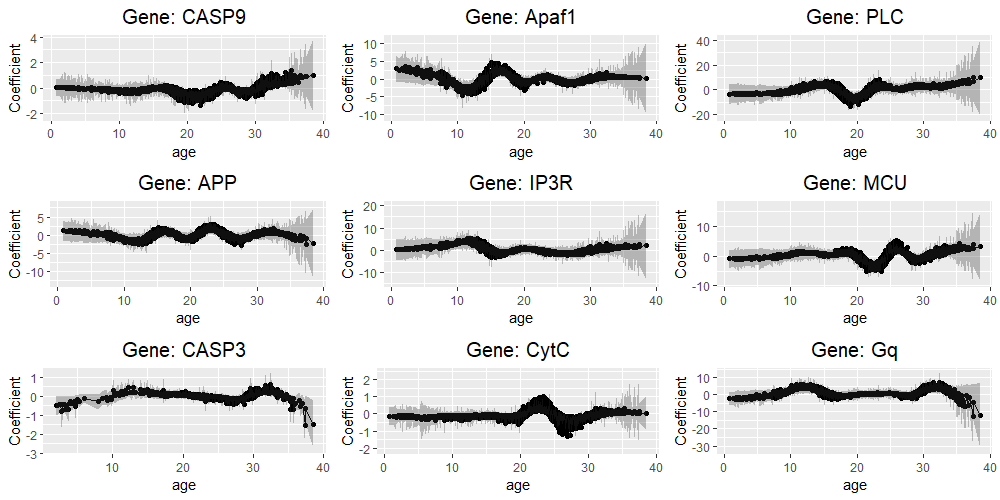
\includegraphics[width=1\textwidth]{Figures/3.4.png} 
%\caption{Main name 2} 
\label{Fig.3.4} 
\end{figure}








